% !TEX encoding = UTF-8 Unicode
% лекции 7-8, 5 марта 2016
% вопросы 12, 14-17
% 12. Принцип максимума для уравнения теплопроводности во всем пространстве. Два следствия.
% 14. Фундаментальное решение для уравнения теплопроводности.
% 15. Интегральная формула для решения  задачи Коши для однородного уравнения теплопроводности в пространстве. Свойства решения.
% 16. Решение задачи Коши для неоднородного уравнения теплопроводности в пространстве. Метод Дюамеля.
% 17. Уравнения Лапласа, Пуассона. Физическая интерпретация (конвективный теплообмен, электростатика).


\subsection{Принцип максимума для уравнения теплопроводности во всем пространстве}
Поставим задачу Коши для однородного уравнения теплопроводности во всем пространстве $\real^n$:
\begin{align}
    \begin{cases} 
        u_t - a^2 \Delta u = 0, \\
        u (0, x) = \varphi (x).
    \end{cases}
\label{heathomcauchy}
\end{align}

\begin{center}
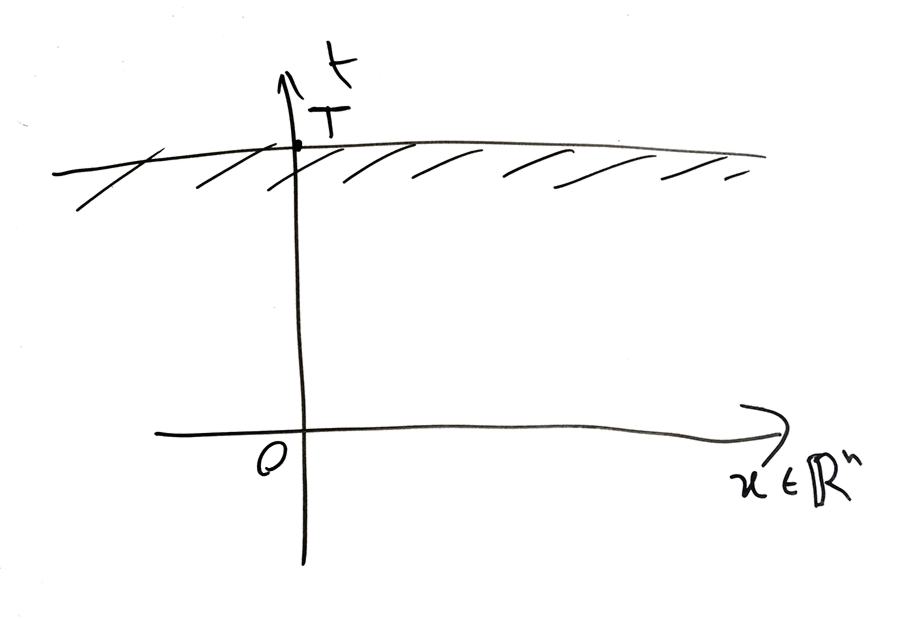
\includegraphics[scale=0.25]{part4.1.png}
\end{center}

Будем рассматривать решения на бесконечных цилиндрах $$u : \real^+ \times \real^n \rightarrow \real,$$ 
ограниченные в каждой ограниченной полосе: 
\begin{equation}
	\forall T > 0 \quad \exists C = C(T) > 0 : \quad |u(t, x)| \leq C(T) \quad \forall t \in [0, T] \quad \forall x \in \real^n.
\label{условие во всем пространстве}
\end{equation}

\begin{theorem}[Принцип максимума для уравнения теплопроводности во всем пространстве]
Пусть поставлена задача Коши для уравнения теплопроводности в $\real^n$ \eqref{heathomcauchy}, и $T > 0$. Тогда для решения, ограниченного в каждой ограниченной полосе верно, что супремум по всей полосе равен супремуму по нижней границе полосы:
$$ M_+ = \sup_{\stackrel{x \in \real^n,} {t \in [0, T]}}u(t,x), \quad N_+ = \sup_{x \in \real^n} u(0, x), \quad M_+ = N_+ $$

\begin{note}
Очевидно, $-\infty < N_+ \leq M_+ < +\infty.$
\end{note}
\end{theorem}

\begin{proof}
Вспомним обозначения для оператора теплопроводности:
$$ Lu = u_t - a^2 \Delta v.$$
Пусть $\eps >0 $ и $u$ - решение уравнения теплопроводности во все пространстве. Рассмотрим
$$v_\eps(t, x) = u(t, x) - \eps(2na^2t + \abs{x}^2).$$
Тогда
$$Lv_\eps = Lu - \eps L(2na^2t + \abs{x}^2) = -\eps(2na^2 - 2n\Delta x^2) = -\eps(2na^2 - 2na^2) = 0.$$
Таким образом, $v_\eps$ --- тоже решение уравнения теплопроводности во всем пространстве.

Рассмотрим открытые цилиндры: $$Q_{T,R} = (0,T)\times B_R(0).$$

\begin{center}
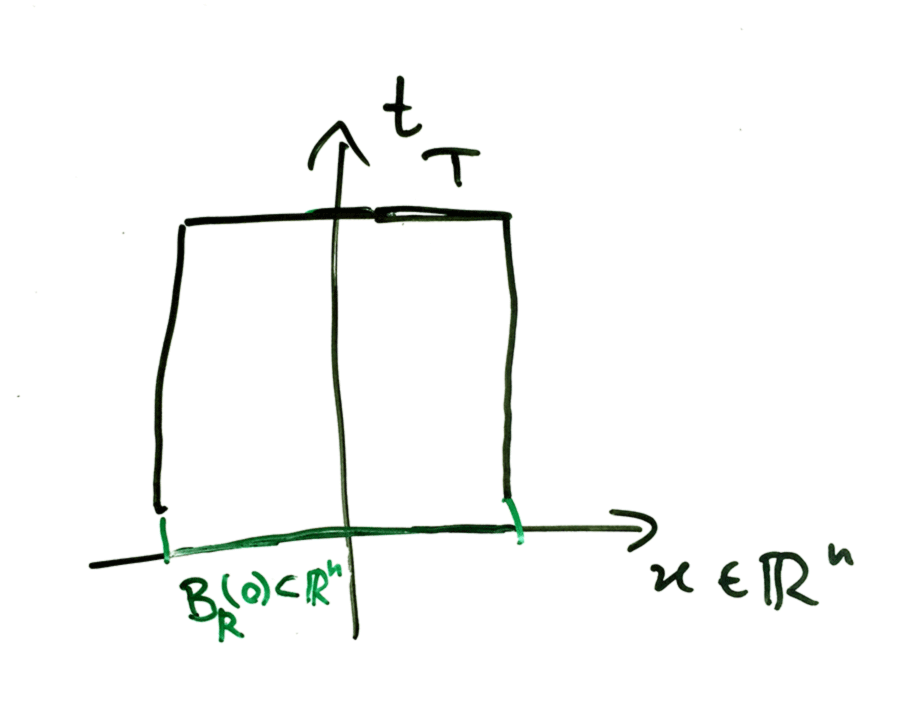
\includegraphics[scale=0.25]{part4.2.png}
\end{center}

Можно заметить, что полоса равна объединению всех таких цилиндров по $R$. По принципу максимума в ограниченной области максимум и минимум достигаются на параболической границе. На нижней крышке имеем
$$ v_\eps (0,x) = u(0,x) - \eps |x|^2 \leq N_+ \quad$$
На боковой поверхности:
$$v_\eps(t,x)\Bigg\rvert_{\abs{x} = R} = u(t,x) \Bigg\rvert_{\abs{x} = R} - \eps(2na^2t + R^2) \leq u(t,x)\Bigg\rvert_{\abs{x} = R} - \eps R^2 \leq M_+ - \eps R^2$$
Для любого $\eps$ можно подобрать такой $R_\eps$, чтобы было верно неравенство $$ M_+ - \eps R^2_\eps \leq N_+.$$

Таким образом,
$$ v_\eps (t, x) \leq N_+ \quad \forall (t,x) \in {Q_{T, R_\eps}}$$
Осталось доказать, что
$$u(t,x) \leq N_+, \quad \forall (t,x) \in [0, T] \times \real^n$$
Фиксируем произвольную точку $(t,x)$. Начиная с какого-то $\eps_0$ она будет лежать в цилиндрах $Q_{T, R_\eps}$, и станет верно
$$v_\eps(t,x) = u(t,x) - \eps(2na^2t - \abs{x}^2) \leq N_+ \quad \forall \eps \geq \eps_0$$
То есть,
$$u(t,x) \leq N_+ + \eps \underbrace{(2na^2t + |x|^2)}_{const}$$
Устремив $\eps$ к нулю, получаем искомое соотношение.

\end{proof}

\begin{corollary}[Принцип минимума для уравнения теплопроводности во всем пространстве]
$$M_- = \inf_{\stackrel{x \in \real^n, \,} {t \in [0, T]}}u(t,x); \qquad N_- = \inf_{x \in \real^n}u(0,x),$$
то $M_-=N_-$ (инфимум по полосе равен инфимуму по нижней границе).
\end{corollary}

\begin{corollary}[Единственность]
Рассмотрим задачу Коши для неоднородного уравнения:
\begin{align}
    \begin{cases} 
        u_t - a^2 \Delta u = q, \\
        u (0, x) = \varphi (x).
    \end{cases}
\label{heatnonhomcauchy}
\end{align}
Классическое решение для задачи \eqref{heatnonhomcauchy} --- единственное в классе функций, ограниченных в каждой полосе.
\end{corollary}

\begin{proof}
Пусть $u_1, \, u_2 $ --- два решения. $L$ --- оператор теплопроводности.  Тогда
\begin{align*}
	\begin{cases*}
		Lu_1 = Lu_2 = q, \\
		u_1\Big\rvert_{t=0} = u_2\Big\rvert_{t=0} = \varphi(x),
	\end{cases*}
	\quad \Rightarrow \quad
	\begin{cases*}
		L(u_1 - u_2) = 0, \\
		\quad (u_1-u_2) \Big\rvert_{t=0}=0.
	\end{cases*}
\end{align*}

Таким образом, $u = u_1 - u_2$ --- решение однородной задачи с нулевыми начальными условиями (в том же классе ограниченных в полосе функций). Значит, по доказанной теореме супремум и инфимум $u$ равны нулю, и, следовательно, $u1 = u2$.

\end{proof}

\begin{note}
Условие ограниченности в каждой полосе необходимо, так как без него решение не будет единственным: кроме решения в полосе будет еще и некое быстрорастущее решение. Неединственность относится уже не к теплопроводности, поэтому физики тоже накладывают ограничения, чтобы получать единственное решение.
\end{note}


\subsection{Фундаментальное решение уравнения теплопроводности}

Хотим получить решение для системы \eqref{heathomcauchy}. Получим --- фундаментальное решение уравнения теплопроводности (в ходе решения будем накладывать некоторые специфические условия на решение).

Рассмотрим $a = 1$ иначе можно сделать замену $x \rightarrow \dfrac{x}{a}$ (делаем это для упрощения вычислений).

\begin{enumerate}
\item $u(t,x) = \lambda^\alpha u(\lambda t, \lambda^\beta x) \quad \forall \lambda$ (т.~е. хотим частичную линейность решения)

Рассмотрим $\lambda = \dfrac{1} {t}. \, \alpha, \, \beta$ --- неизвестны.
$$u(t,x) = \dfrac{1}{t^\alpha}(1, \dfrac{x}{t^\beta}) \text{. Обозначим } \, u(1,z) = v(z) \Rightarrow u(t,x) = \dfrac{1}{t^\alpha} v(\dfrac{x}{t^\beta}).$$
Посчитаем $Lu = 0$:
$$-\dfrac{\alpha}{t^{\alpha + 1}} v\left( \dfrac{x}{t^\beta}\right) - \dfrac{\beta}{t^{\alpha + \beta + 1}}\nabla v\left( \dfrac{x}{t^\beta}\right)\cdot x - \dfrac{1}{t^\alpha t^{2\beta}}\Delta v\left( \dfrac{x}{t^\beta}\right) = 0.$$
$$\left(\text{т.к.} \, \dfrac{\partial}{\partial t} \left(v\left( \dfrac{x}{t^\beta}\right)\right) = \sum \dfrac{ \partial v}{\partial x_i}\left(\dfrac{x}{t^\beta}\right) \cdot \dfrac{-\beta x_i}{t^{\beta + 1}} = -\dfrac{\beta}{t^{\beta + 1}}\nabla v\left( \dfrac{x}{t^\beta}\right) \cdot x \right)$$

Сделаем замену $ y = \dfrac{x} {t^\beta}.$
$$ \dfrac{\alpha}{t^{\alpha + 1}} v(y) + \dfrac{\beta}{t^{\alpha + 1}} \nabla v(y) \cdot y + \dfrac{1}{t^\alpha  t^{2\beta}}\Delta v(y)=0.$$

Пусть $\beta = \dfrac{1}{2}$ и умножаем полученное выражение на $t^{\alpha + 1}:$
$$\alpha v(y) + \dfrac{1}{2} \nabla v(y) \cdot y + \Delta v(y) = 0.$$

\item $u(t,x) = \tilde{u}(t,|x|)$ --- хотим симметрии относительно 0, т.~о. $v(y) = w(|y|), |y| = r.$ Тогда получим:
$$ \alpha w(r) + \dfrac{1}{2} w'(r) \cdot r + w''(r) + \dfrac{n}{r}w'(r) = 0;$$
$$\text{т.~к.} \quad \Delta v(y) = \dfrac{\partial^2v}{\partial y_1^2} + \dots + \dfrac{\partial^2v}{\partial y_n^2};$$
$$\dfrac{\partial w}{\partial y_i} = w' \dfrac{\partial |y|}{\partial y_i} = w' \dfrac{y_i}{r} \Rightarrow 
\dfrac{\partial^2 w}{\partial y_i^2} = w''\dfrac{y_i^2}{r^2} + w'\left(\dfrac{1}{r} - \dfrac{y_i^2}{r^2}\right) \Rightarrow$$
$$\Delta w(r) = \dfrac{w''}{r^2}\sum y_i^2 + \dfrac{w'}{r}\sum (1 - \dfrac{y_i^2}{r^2}) = w'' + \dfrac{w'n}{r}.$$

Пусть $\alpha = \dfrac{n}{2}.$
$$\dfrac{n}{2}w(r) + \dfrac{1}{2}w'(r) \cdot r + w''(r) + \dfrac{n-1}{r}w'(r) = 0 \Rightarrow$$$$ \dfrac{1}{2}\left(r^nw\right)' + \left(r^{n-1}w'\right)' = 0 \Rightarrow \dfrac{1}{2}\left(r^nw\right)+ \left(r^{n-1}w'\right) = \gamma.$$

\item $r^aw_n' + r^bw \rightarrow 0 \, \text{при} \, n \rightarrow \infty$ --- хотим, чтобы это выполнялось, такое возможно только при $\gamma = 0,$ т.~о.
$$r^{n-1}w_r' + \dfrac{1}{2}r^nw = 0 \Rightarrow w_r' + \dfrac{r}{2}w = 0 \Rightarrow$$
$$\dfrac{dw}{w} = -\dfrac{r}{2}dr \Rightarrow w = be^{-\dfrac{r^2}{4}},$$
$$\text{т.~о.} \, u(t,x) = \dfrac{1}{\sqrt{t^n}}u\left(1, \dfrac{x}{\sqrt{t}}\right) = \dfrac{1}{\sqrt{t^n}}w\left(\dfrac{x}{\sqrt{t}}\right) = \dfrac{b}{\sqrt{t^n}}e^{-\dfrac{|x|^2}{4t}}.$$

Получили однопараметрическое семейство решений.
\begin{note}
Если зафиксируем $t$, то полученное выражение --- гауссова функция(нормальное распределение)
%TODO: вставитьрисунок
[рисунок]

,чем $t$ меньше, тем выше "пика" на графике, соответственно, чем больше, тем более сглаженным будет график.
\end{note}
Теперь определенным образом выберем константу, пусть $b\,:\,b>0; \, \int\limits_{\real^n} u(t,x)dx = 1.$

\begin{exercise}
Нужно уметь вычислять $b$.
\end{exercise}

$$b = \dfrac{1}{(4\pi)^{n/2}} \Rightarrow$$$$ u(t,x) = \dfrac{1}{(4\pi t)^{n/2}} \exp\left(-\dfrac{|x|^2}{4t}\right) = \Phi(t,x) \,\text{--- фундаментальное решение уравнения теплопроводности.}$$
\begin{exercise}
Что, если $a \not= 1$?
\end{exercise}
\end{enumerate}

\begin{theorem}[Интегральная формула для решения задачи Коши]
$ \varphi\in C_b(\real^n)$ --- ограниченная и непрерывная(начальное распределение). Тогда
$$u(t,x) = \int\limits_{\real^n}\Phi(t, x-y)\varphi(y)dy (= \left(\Phi(t,\cdot)*\varphi\right)(x) \text{ --- свертка.})$$

\begin{enumerate}
\item $u \in C^\infty\left(\left(0, +\infty\right)\times \real^n\right);$
\item $ u_t - \Delta u = 0$ --- т.~е. решение уравнения теплороводности;
\item $\lim\limits_{(t,\,y) \rightarrow (0,\,x)}u(t,x) = \varphi (x).$
\end{enumerate}

\end{theorem}

\begin{note}[Физический смысл фундаментального решения] %%%слишком много сказано, нужно ли писать, вроде смысла нет.
$\Phi$ - распределение температуры от единичного источника (источник с температурой единица), сосредоточенного в одной точке.
\end{note}
\begin{proof}
\begin{enumerate}
\item $\Phi \in  C^\infty\left(\left(0, +\infty\right)\times \real^n\right)$ --- очевидно.
$$u_t = \int\limits_{\real^n} \Phi_t(t,x-y)\varphi(y)dy, \qquad u_{x_i} = \int\limits_{\real^n} \Phi_{x_i}(t, x-y)\varphi(y)dy$$

Очевидно, $u \in C^\infty.$
\item $Lu = u_t - \Delta u = \int\limits_{\real^n} \underbrace{(\Phi_t - \Delta \Phi)(t, x-y)}_{0}\varphi(y) dy = 0.$
\item Пусть $x_0 \in \real^n.$
$$|u(t,x) - \varphi(x_0)| = \Bigl|\int\limits_{\real^n}{\Phi(t,x-y)\varphi(y)dy} - \varphi(x_0)\Bigl| = \Bigl|\int\limits_{\real^n}\Phi(t,x-y)\varphi(y)dy - \varphi(x_0)\int\limits_{\real^n}\Phi(t,x-y)dy\Bigl|=$$
$$=\Bigl|\int\limits_{\real^n}\Phi(t,x-y)(\varphi(y) - \varphi(x_0))dy\Bigl| \leq \int\limits_{\real^n}\Phi(t,x-y)\bigl|\varphi(y) - \varphi(x_0)\bigl|dy = $$
$$= \underbrace{\int\limits_{B_\delta(x_0)}\Phi(t,x-y)\bigl|\varphi(y) - \varphi(x_0)\bigl|dy}_{I_\delta} + \underbrace{\int\limits_{\real^n \setminus B_\delta(x_0)}\Phi(t,x-y)\bigl|\varphi(y) - \varphi(x_0)\bigl|dy}_{J_\delta}.$$

Пусть $\eps > 0.$ Выберем такое $\delta,$ что $\bigl|\varphi(y) - \varphi(x_0)\bigl|<\dfrac{\eps}{2}$ при $y \in B_\delta(x_0)$ (Такое $\delta \, \exists,$ т.~к. $\varphi$ --- непрерывна).

Тогда $I_\delta \leq \dfrac{\eps}{2}, \, \text{т.к.} \int\limits_{\real^n}\Phi = 1.$

Пусть $|x - x_0| < \dfrac{\delta}{2}, \, y \notin B_\delta(x_0) \Rightarrow |x - y| \geq \dfrac{1}{2}|x_0 - y|.$
$$J_\delta \leq 2||\varphi||_\infty \cdot \int\limits_{\real^n \setminus B_\delta(x_0)} \Phi(t,x-y)dy = 2||\varphi||_\infty \dfrac{1}{(4\pi t)^{n / 2}} \int\limits_{B_{\delta}^c} e^{-\dfrac{|x-y|^2}{4t}}dy \leq $$$$\leq 2||\varphi||_\infty \dfrac{1}{(4\pi t)^{n / 2}} \int\limits_{B_{\delta}^c} e^{-\dfrac{|x_0-y|^2}{16t}}dy \leq \dfrac{C}{(4\pi t)^{n / 2}} \int\limits_\delta^{+\infty} e^{-\dfrac{\rho^2}{16t}}\rho^{n-1}d\rho =  $$$$ = C\int\limits_{\delta / \sqrt{t}}^{+\infty} e^{-\dfrac{\rho^2}{16t}}\rho^{n-1}d\rho \stackrel{t\rightarrow 0}{\longrightarrow} 0$$
$$\delta: \, t < \dfrac{\delta}{2}, \, J_\delta \leq \dfrac{\eps}{2}, \Rightarrow I = I_\delta + J_\delta \leq \eps, \, |x-x_0| < \dfrac{\delta}{2}, \, 0<t<\dfrac{\delta}{2} \Rightarrow $$$$ |u(t,x) - \varphi(x_0)|<\eps$$
\end{enumerate}
\end{proof}

\subsection{Решение задачи Коши для неоднородного уравнения теплопроводности в пространстве. Метод Дюамеля}
\begin{align}
    \begin{cases} 
        u_t - \Delta u = f, \\
        u (0, x) = \varphi (x).
    \end{cases}
\label{heatnonhomcauchy2}
\end{align}
$t \in \real^+,\, x \in \real^n, f=f(t,x)$

\begin{note}

Достаточно решать для случая $\varphi = 0, \, f \not= 0 \, \text{и} \, \varphi \not=, \, f = 0,$ т. е. пусть $u_1, \, u_2 :$
\begin{equation*}
\begin{cases} 
        Lu_1 = f, \\
        u_1\Bigl|_{t=0} = 0.
    \end{cases}
    \qquad
    \begin{cases} 
        Lu_2 = 0, \\
        u_2\Bigl|_{t=0} = \varphi (x).
    \end{cases}
\end{equation*}
Тогда $u = u_1+u_2:$
\begin{align}
\begin{cases} 
        Lu = f, \\
        u\Bigl|_{t=0} = \varphi (x).
    \end{cases}
    \end{align}
\end{note}

{\itshape Принцип Дюамеля.} Пусть $\varphi = 0$
\begin{equation*}
v(t,x,s) : \quad
    \begin{cases} 
        v_t - \Delta v = 0, \\
        v\Bigl|_{t=s} = f(s, \,).
    \end{cases}
\end{equation*}
$$u(t,x) = \int\limits_0^tv(t,x,s)ds = \int\limits_0^t ds \int\limits_{\real^n}\Phi(t-s, x-y)f(s,y)dy.$$

\begin{theorem}
Пусть $ u(t,x) = \int\limits_0^t ds \int\limits_{\real^n}\Phi(t-s, x-y)f(s,y)dy,$ тогда при $f\in C_x^2, \, C_t^1, f $ --- финитная $\in C_0^\infty( (0,+\infty) \times \real^n),$
\begin{enumerate}
\item $u \in C_t^1, \, u \in C_x^2;$
\item $u_t(t,x) - \Delta u(t,x) = f, \, u(0,x) = 0;$
\item $\lim u(t,x) = 0$ при $(t,x) \rightarrow (0,x_0) \forall x_0 \in \real^n.$
\end{enumerate}
\end{theorem}

\begin{proof}

$$u(t,x) = \int\limits_0^t ds \int\limits_{\real^n} \Phi(s,y)f(t-s, x-y)dy \, \text{--- свертка},$$ т.к. $f\in C_x^2, \, C_t^1, f $ --- финитная и $\Phi(s,y)$ гладкая в окрестности $s = t >0:$
$$\dfrac{\partial^2u}{\partial x_i^2} = \int\limits_0^t ds \int\limits_{\real^n} \Phi(s,y)f_{x_i x_i}(t-s, x-y)dy;$$
$$u_t = \int\limits_{\real^n} \Phi(t,y)f(0,x-y)dy + \int\limits_0^t ds\int\limits_{\real^n} \Phi(s,y)f_t(t-s, x-y)dy,$$ т.е. $u \in C_t^1, \, u \in C_x^2.$

$$u_t - \Delta u = \int\limits_{\real^n} \Phi(t,y)f(0,x-y)dy + \int\limits_0^t ds\int\limits_{\real^n} \Phi(s,y)f_t(t-s, x-y)dy-$$$$ - \int\limits_0^t ds \int\limits_{\real^n}dy\underbrace{\sum \Phi(s,y)f_{x_i x_i}(t-s, x-y)}_{\Phi(s,y)\Delta f(t-s, x-y)} = $$
$$= \int\limits_{\real^n} \Phi(t,y)f(0,x-y)dy + \int\limits_0^t ds \int\limits_{\real^n}dy \Phi(s,y)(-\dfrac{\partial}{\partial s} - \Delta y) = $$ $$= \underbrace{ \int\limits_0^\eps ds \int\limits_{\real^n}\Phi(s,y)\left(\left(-\dfrac{\partial}{\partial s} - \Delta y\right)f(t-s, x-y)\right)dy}_{I_\eps} + \underbrace{\int\limits_{\real^n} \Phi(t,y)f(0,x-y)dy}_{k} + $$
$$+ \underbrace{\int\limits_\eps^t ds \int\limits_{\real^n} \Phi(s,y)\left(\left(-\dfrac{\partial}{\partial s} - \Delta y\right)f(t-s, x-y)\right)dy}_{J_\eps}.$$
$$\abs{I_\eps} \leq \left(||f_t||_\infty + ||\Delta_x f||_\infty\right)\int\limits_0^\eps ds \int\limits_{\real^n}\Phi(s,y)dy = C\eps.$$
$$J_\eps = \int\limits_\eps^t ds \underbrace{\int\limits_{\real^n}\left(\left(\dfrac{\partial}{\partial s} - \Delta y\right)\Phi(s,y)\right)f(t-s, x-y)dy}_{0, \, \text{т.к.} \, \Phi \, \text{--- решение однородного уравнения}} + \int\limits_{\real^n} \Phi(\eps, y)f(t-\eps, x-y)dy - $$ $$-\underbrace{\int\limits_{\real^n} \Phi(t,y)f(0,x-y)dy}_{\text{это} \, k}.$$
При $\eps \rightarrow 0:$
$$u_t - \Delta u = \lim_{\eps \rightarrow 0} \int\limits_{\real^n}\Phi(\eps, y)f(t-\eps, x-y)dy = \lim_{\eps \rightarrow 0} \int\limits_{\real^n}\Phi(\eps, x-y)f(t-\eps, y)dy = f(t,x) \Rightarrow$$ $\Rightarrow u$ --- решение.

$$\abs{u(t,x)} \leq \int\limits_0^t ds \int\limits_{\real^n}\Phi(s,y)\underbrace{\abs{f(t-s, x-y)}}_{\leq C, \, \text{т.к. финитная}}dy \leq C\int\limits_0^t ds \int\limits_{\real^n}\Phi(s,y)dy = Ct \stackrel{t \rightarrow 0} \longrightarrow 0. $$
\end{proof}

\subsection{Уравнения Лапласа и Пуассона}

Уравнение Лапласа: \begin{align}-\Delta u = 0, \, u = u(x), \, x \in \Omega \subset \real^n.\label{Laplace}\end{align}
Уравнение Пуассона: \begin{align}-\Delta u = f, \, f = f(x).\label{Poisson}\end{align}

{\itshape Физическая интерпретация.} Описывают стационарное температурное поле в области $\Omega$, в которой плотность источников и стоков теплоты не зависит от $t$.

Из закона Гаусса: $\overrightarrow{div}E = q(x),$ где $E$ --- напряженность электростатического поля, $q(x)$ --- плотность заряда.
Потенциал электростатического поля $\varphi:$
$$\stackrel{\rightarrow} E = -\nabla \varphi;$$
$$-\overrightarrow{div}\nabla\varphi = q;$$
$-\Delta \varphi = q$  --- уравнение для распределения потенциала электростатического поля с плостностью зарядов $ q.$

Основные задачи:
\begin{enumerate}
\item Задача Дирихле
$$\varphi \Bigl|_{\partial\Omega} = g.$$
В случае теплообмена: задана температура на границе; в случае электростатики: задан потенциал на границе.
\item Задача Неймана
$$\dfrac{\partial\varphi}{\partial n}\Bigl|_{\partial\Omega}=0.$$
Идеально изолированная область.
\end{enumerate}
